\documentclass[a4paper,10pt]{report}

\usepackage[latin1]{inputenc}
\usepackage{amsmath}
\usepackage{amsfonts}
\usepackage{amssymb}
\usepackage{graphicx}
\usepackage[catalan]{babel}
\usepackage{fancyhdr}

% Salto de l�nea tras t�tulo de secciones \paragraph
\makeatletter % necesario para que reconozca a '@' como car�cter normal
\renewcommand{\paragraph}{\@startsection{paragraph}{4}{\z@}{-3.25ex \@plus -1ex \@minus -.2ex}{1.5ex \@plus .2ex}{\normalfont\normalsize\bfseries}}
\makeatother % necesario para que restablezca '@' como car�cter especial


% Title Page
\author{
  Albert Farr�s Coma
  \and
  Jonathan Mart� Fraiz
  \and
  C�sar P�rez Laguna
  \and
  Llu�s Vilanova Garc�a
}

\title{
  \textbf{
  Arquitectura Transparent \\
  per a l'Administraci� de Cl�sters
  }
}


\begin{document}
\maketitle

\tableofcontents

% Cabeceras
\pagestyle{fancy}
%\fancyhf{} % borrar todos los ajustes
% En lo siguiente, fancyhead sirve para configurar la cabecera, fancyfoot para
% el pie.
% Justificaci�n: C=centered, R=right, L=left, (nada)=LRC
% P�gina: O=odd, E=even, (nada)=OE
\fancyhead[]{}  % n�mero de cap�tulo
\fancyhead[L]{\leftmark}  % n�mero de cap�tulo
%\fancyhead[R]{\thepage} % n�mero de p�gina
% Modifica el ancho de las l�neas de cabecera y pie
\renewcommand{\chaptermark}[1]{
	\markboth{\chaptername\  \thechapter. #1}{}
}
\renewcommand{\headrulewidth}{0.4pt}

\chapter{Qu� i perqu� ho volem fer?}

El que pretenem fer �s una interf�cie per al control i administraci� d'un
sistema de clustering a trav�s del sistema de fitxers.

Per exemple, per migrar un proc�s d'un node a un altre, seria tan f�cil com
moure un fitxer d'un directori a un altre (representant cada directori un node
diferent i cada proc�s representat per un fitxer) amb el navegador de fitxers
preferit.

D'aquesta manera l'usuari no ha de tenir coneixements sobre com funcionen les
eines de clustering que li ofereix el sistema on treballa, de forma que
l'abstracci� que proposem li permeti treballar amb diferents sistemes des d'una
interf�cie comuna.

Hem anomenat al sistema TACA, que ve de l'angl�s Transparent Architecture for
Cluster Administration (Arquitectura Transparent per a l'Administraci� de
Cl�sters).

Tant la documentaci� com la implementaci� es troben disponibles a la p�gina del
projecte, que es troba a \textbf{http://developer.berlios.de/projects/taca}.


\chapter{Conceptes b�sics}

\section{Clustering}

\subsection{Introducci�}

En termes generals un cluster �s un grup de sistemes independents que treballen
junts com un sistema �nic. El client interactua amb un cluster com si f�s un
servidor �nic. Les configuracions de cluster s'utilitzen per a tenir
disponibilitat i escalabilitat:

\begin{description}
\item[Disponibilitat:]
Quan un sistema falla en el cluster, el programari del cluster respon
distribuint el treball del sistema que ha fallat als sistemes que queden en el
cluster.

\item[Escalabilitat:]
Quan la c�rrega general excedeix les capacitats dels sistemes en el cluster, �s
possible afegir sistemes addicionals al mateix.  En l'actualitat, els clients
que planegen ampliar la capacitat del seu sistema han de considerar servidors
"high end" costosos que proporcionen espai per a CPUs, controladors i mem�ria
addicionals. Al utilitzar la tecnologia de clustering, els clients podran
afegir gradualment sistemes est�ndards m�s petits, segons sigui necessari, per a
satisfer els requeriments generals de pot�ncia de processament.
\end{description}


\subsection{Diferents implementacions}
A continuaci� passarem a descriure per sobre algunes de les diferents
implementacions existents en alguns sistemes operatius, les quals representen
diferents paradigmes.


\subsubsection{Linux}

\begin{itemize}
\item \textbf{OpenMosix:}
�s una implementaci� basada en la distribuci� de processos, com a modificaci�
per al nucli, de forma que el proc�s �s totalment transparent a l'usuari (al
programador* de l'aplicaci�), cosa que fa molt m�s portables els programes a
d'altres sistemes, utilitzin o no OpenMosix, i des d'aplicacions no dissenyades
espec�ficament per a executar-se en un cluster.

De totes maneres, per tal de poder paral�lelitzar les aplicacions, aquestes han
d'haver estat ja programades amb diversos processos, ja que OpenMosix no
paral�lelitza aplicacions, sin� que nom�s distribueix la c�rrega entre els
diferents nodes.

Per exemple, si tenim deu nodes al cluster i executem un programa (amb un sol
proc�s), tardar� el mateix que si nom�s tingu�ssim un node; per� si executem deu
programes d'aquests, tardaran el que si nom�s n'execut�ssim un, ja que cadascun
s'executar� en un node.

Un inconvenient, per�, �s que tots els nodes del cluster han de tenir exactament
el mateix nucli (sense compatibilitat de versions ni cap endavant ni cap
enrere).

Un altre dels problemes de OpenMosix, �s que no pot migrar cap proc�s que
comparteixi mem�ria, de forma que tampoc podr� migrar threads, ja que aquests
comparteixen mem�ria.


\item \textbf{Beowulf:}
\nocite{Beowulf-Home}
\nocite{Beowulf-Howto}
Beowulf, segons una de les definicions que hem trobat (doncs alguns diuen que es
pot dir que un sistema �s Beowulf nom�s si est� constru�t de la mateixa forma que
la m�quina original de la NASA; d'altres van cap a l'altre extrem i diuen que �s
un sistema Beowulf tot aquell conjunt de m�quines que corren codi paral�lel), �s
una arquitectura multi-computador que pot ser utilitzada per a fer computacions
en paral�lel. Normalment consisteix en un node servidor i un o m�s nodes
connectats via Ethernet (o qualsevol altre xarxa), per� el millor de tot �s que
es pot construir amb hardware "normal", com per exemple qualsevol PC que pugui
utilitzar Linux, adaptadors est�ndard d'Ethernet i switchos. Beowulf tamb�
utilitza software "com�", com el sistema operatiu Linux, PVM (Parallel Virtual
Machine) i MPI (Message Passing Interface). Una de les grans difer�ncies entre
Beowulf i un cluster de estacions de treball (COW - Cluster of Workstations) �s
el fet de qu� Beowulf es comporta com una �nica m�quina m�s que no mas com un
conjunt d'estacions de treball. Els nodes de Beowulf es poden pensar com un
paquet de CPU + mem�ria que es pot connectar al cluster, tal com una CPU o un
m�dul de mem�ria es poden connectar a una placa base.

Beowulf no �s un paquet de software especial, una nova topologia de xarxa o
l'�ltim hack per al kernel, sin� que �s una tecnologia de clustering de m�quines
Linux per a formar un supercomputador paral�lel virtual. Tot i que hi ha varis
paquets de software com modificacions per al kernel, llibreries PVM i MPI i
eines de configuraci� que fan l'arquitectura Beowulf m�s r�pida, m�s f�cil de
configurar i molt m�s usable, un pot constru�r una m�quina de la classe Beowulf
utilitzant distribucions de Linux est�ndards sense cap software addicional.
Tenint un parell de m�quines linux en xarxa que comparteixen com a m�nim el
/home a trav�s de NFS i es confien l'una a l'altra per executar shells remotes
(rsh), es podria dir que es t� una m�quina Beowulf molt simple de dos nodes.

Aix� doncs, est� clar que una aplicaci�, per a funcionar en una arquitectura
Beowulf, ha d'haver estat escrita utilitzant llibreries o m�todes
especialitzats, no transparents a l'usuari, per� ofereix m�s rendiment que, per
exemple, OpenMosix (tot i que aquest �ltim �s totalment transparent a l'usuari).



\item \textbf{Altre software de clustering:}
Tot i buscar per Internet la exist�ncia d'altre software de clustering, no hem trobat res excepte distribucions basades en el software que ja hem comentat.
\end{itemize}


\subsubsection{Microkernels (Mach/L4)}

No existeix cap eina suficientment madura sobre microkernels que ens ofereixi
tot el que tenim en altres sistemes com Linux. Tot i aix� si que es poden
trobar alguns projectes d'investigaci� que fan refer�ncia a la construcci� de
sistemes de clustering sobre microkernels. Hem trobat dos exemples:

Hurricane Operating System, cl�ster experimental orientat a la investigaci� i
la recerca \cite{Microkernel-HOS}.

CHORUS/Fusion per SCO Sopen Menystens Software is una implementaci�
multi-servidor per SCO UNIX. Aquest entend SCO Unix amb funcionalitats de
temps real i clustering.


\subsubsection{Altres Sistemes Operatius}

\begin{itemize}
\item {\textbf{Solaris:}}
Hem trobat exemples de cl�sters de computaci� constru�ts amb aquest Sistema
Operatiu, per exemple, el SciClone Cluster Project \cite{AltresSO-SciCLone}.
El cl�ster est� format exclusivament per m�quines Sun per� no donen moltes
caracter�stiques del sistema operatiu, ni tampoc si han tingut que desenvolupar
un afegit per dona suport per clustering.

\item {\textbf{MacOSX:}}
Utilitzant la bibloteca de processament carbonlib m�s un software de clustering
anomenat pooch \cite{AltresSO-MacOS} es pot crear un cluster amb
aquest sistema operatiu. Com passa a Beowulf per Linux, aquest sistema de
clustering est� basat en l'�s de biblioteques de paral�leliitzaci� i per tant
els programes s'hauran d'escriure pensant que s'executen en un cluster no �s
transparent a l'usuari/aplicaci�.
\end{itemize}


\section{Abstraccions existents en Sistemes de Fitxers}

\subsection{Translators de Hurd}
\nocite{Hurd-Translators}
Els translators s�n servidors de Hurd (SO basat en el micronucli gnuMach, tot i
que s'est� migrant cap a oskit-Mach i, en un futur, cap a L4) que proporcionen
la interf�cies b�sica del sistema de fitxers, de manera que es poden inserir
entre el contingut real d'un fitxer (entenent com a fitxer la representaci�
corresponent en el sistema de fitxers - inode -, doncs el fitxer real pot estar
en una altra m�quina o, fins i tot, no ser cap fitxer, sin� la representaci�
d'una zona de mem�ria) i l'usuari que accedeix al fitxer, de forma que
\textit{tradueix} les peticions de l'usuari.

Els translators, a m�s am�s, tenen unes propietats molt interessants, i �s que
des del punt de vista del kernel, no s�n m�s que processos d'usuari, de forma
que els pot executar qualsevol usuari, sense necessitat de tenir permisos de
superusuari per instal�lar o modificar un translator, l'�nic que fa falta �s
tenir drets d'acc�s a l'inode sobre s'uneix el translator. Molts translators no
requereixen un fitxer per a funcionar, i �s per aix� que la informaci� sobre
aquests es guarda a l'inode.

Els translators s�n responsables de servir totes les operacions del sistema de
fitxers que fan refer�ncia a l'inode al que s'uneix. Per aix�, al no estar
restringits al t�pic conjunt d'objectes (fitxer de dispositiu, link, etc.), s�n
lliures de retornar qualsevol cosa que tingui sentit per al programador.  Un
exemple podria ser un translator que es comport�s com un directori quan fos
accedit per \texttt{cd} o \texttt{ls} per� que al mateix temps es comport�s com
un fitxer al ser accedit per \texttt{cat}.


\subsection{/proc de Linux}

\subsubsection {Introducci� a /proc}

Linux mant� una abstracci� de sistema de fitxers virtual anomenada /proc. En
diem abstracci�, perqu� realment no �s ben b� un sistema de fitxers implementat
sobre VFS com ho poden ser: Ext2, Ext3, ReiserFS, Minix...
A m�s /proc en podem dir que �s un pseudo-sistema de fitxers, ja que en realitat
cap dels fitxers o directoris que s'hi visualitzen existeixen realment.

/proc �s realment un mirall on s'hi veuen reflectides algunes de les
estructures del nucli del sistema operatiu, i per mitj� del qual podem
controlar alguns par�metres de seguretat tan f�cilment com resulta interactuar
amb sistema de fitxers real.


\subsubsection {M�s sobre /proc}

/proc est� disponible en el sistema operatiu Linux quan el nucli es compila amb
la opci� CONFIG\_PROC\_FS=Y. Tamb� haurem de seleccionar la opci�
CONFIG\_SYSCTL=Y per a poder modificar el valor de determinats par�metres.
La majoria de distribucions inclouen nuclis compilats amb aquesta opci� i en
general �s aconsellable seleccionar-la en el moment de recompilar el nucli.

\subsubsection {Com es munta?}

El pseudo-sistema de fitxers /proc es pot muntar autom�tic en el moment
d'iniciar el sistema indicant-ho a /etc/fstab. En el cas que sigui necessari
muntar-lo manualment utilitzar�em la seg�ent comanda:

\begin{quotation}
\verb"mount -t proc proc /proc"
\end{quotation} 

�s aconsellable que /proc sigui muntat autom�ticament al sistema.
En cas de no disposar del suport per a /proc, alguns programes d'administraci�
del sistema (com per exemple el que nosaltres estem desenvolupant) no
funcionaran ja que no podrem modificar/accedir en temps d'execuci� a alguns
par�metres del nucli del sistema operatiu (molts d'ell de seguretat).

\subsubsection {Qu� cont� /proc?}
Dins del directori /proc hi trobem dos tipus b�sics d'informaci�.
En primer lloc, per a cada proc�s actiu existeix un directori.
Dins del directori de cada proc�s hi ha diversos fitxers aix� com un
subdirectori d'informaci� espec�fica del proc�s (par�metres passats per l�nia de
comandes, enlla� al directori actual del proc�s, variables d'entorn dins del
context del proc�s, els descriptors de fitxers oberts pel proc�s, mapa i
informaci� sobre la utilitzaci� de la mem�ria...).

Adicionalment, existeixen una s�rie de directoris amb informaci� sobre els
diferents m�duls del sistema operatiu. O tal i com veurem en aquest treball,
OpenMosix proporciona un subdirectori (hpc) dins de /proc en el qual hi trobarem
alguns fitxers que ens seran de gran utilitat per a implementar les
funcionalitats que defineixen el nostre projecte.

Al fitxer proc.txt (disponible al directori de documentaci� de sistemes de
fitxers del codi font del nucli de Linux) hi ha informaci� detallada de tot el
que podem trobar dins de /proc.
Un altre document d'inter�s �s ip-sysctl.txt, disponible al directori de
documentaci� sobre treball en xarxa.

No tots els par�metres existents en /proc s�n modificables directament per
l'usuari. De fet, la majoria s�n valors de nom�s lectura i altres s�n molt
millor controlar-los per mitj� del nucli amb la utilitzaci� de les divers
funcions i eines existents al sistema.


\subsubsection {Exemples de directoris}
/proc/sys/net/ipv4 

Dins d'aquest directori tenim disponibles una s�rie de fitxers amb els valors i
par�metres del protocol IP versi� 4. Es tracta d'una s�rie de valors directament
emprats pel nucli del sistema operatiu en les comunicacions TCP/IP basades en el
protocol IP versi� 4.

Per determinar el valor d'algun d'aquests par�metres, l'�nica cosa que hem de
fer �s mirar el seu contingut. Per exemple:

\begin{quotation}
\verb"$ cat /proc/sys/net/ipv4/icmp_echo_ignore_all"

\verb"0"
\end{quotation} 

Ens mostra que actualment el sistema operatiu t� assignat el valor 0
(desactivat) al par�metre ICMP\_ECHO\_IGNORE\_ALL.

L'usuari \textit{root} del sistema t� el privilegi de modificar el valor
d'aquesta variable:

\begin{quotation}
\verb"# echo 1 > /proc/sys/net/ipv4/icmp_echo_ignore_all"
\\
\verb"# cat /proc/sys/net/ipv4/icmp_echo_ignore_all"

\verb"1"
\end{quotation} 

M�s endavant, als apartats d'implementaci� amb OpenMosix, veurem com tamb�
podr�em editar par�metres de fitxers del subdirectori que ofereix per a
realitzar algunes de les funcions que ens proporciona (ex: Bloquejar un node per
rebre processos remots)


\subsection{Altres abstraccions en SFs}

Com que en Linux tots els sistemes de fitxers, virtuals i no virtuals, estan basats en el VFS, no hem trobat res en aquest sistema.

Emper� tampoc hem trobat res en d'altres sistemes, excepte els translators que ja hem comentat per a GNU/Hurd, de manera que no hem aconseguit trobar res per encabir en aquesta secci�.
\begin{document}

\chapter{Software de clustering existent}

\section{Necessitats generals}
(qu� ens ha d'oferir la capa inferior) \\
(poder migrar processos, poder veure on s�n, ...) \\
(qu� nosaltres VOLEM poder fer)

\subsection {A nivell de cluster...}
\begin{itemize}
\item Consultar quantitat de nodes del cluster
\item Consultar carrega total del cluster
\end{itemize}

\subsection {A nivell de node...}
\begin{itemize}
\item Quantitat de CPU's d'un node
\item Consultar carrega del node
\item Consultar estat de memoria
\item Bloquejar l'arribada de nous processos remots
\item Bloquejar la migracio de processos locals
\item Activar/Desactivar la migraci� automatica de processos
\item Demanar que els processos que ha creat un node i han migrat, tornin  a
aquest node (come back home)
\item Expulsar els "processos convidats" a casa
\item Saber quin identificador te un node
\item Modificar/Consultar la velocitat d'un node
\item Consultar informacio de processos (resum de l'estat de processos locals, i
remots)
\item Consultar resum de l'estat del node
\end{itemize}

\subsection {A nivell de proces...}
\begin{itemize}
\item Moure processos d'un node a un altre
\item Bloquejar un proces en un node concret (/proc.....lock)
\item Crear un nou proces en una maquina (crear un fitxer)
\item Matar un proces (esborrar un fitxer)
\item Copiar un proces??
\item Modificar/veure memoria del proces (/proc....mem)
\item Consultar la linia de comandes amb la que s'ha ex/proc....cmdline)
\item Consultar estat del proces (/proc....status)
\item Consultar quants cops s'ha migrat el proces
\item Consultar on s'esta computant actualment
\item Consultar quin node el va crear
\item Saber l'identificador de proces (ID global)
\item Saber l'identificador local d'un proces (ex: PID)
\item Consultar resum de us de CPU
\item Consultar resum de us de Memoria
\end{itemize}


\section{Qu� ens ofereixen els sistemes}
(qu� proporciona a una capa superior) \\
(si ja proporciona una abstracci� semblant a la que volem...) \\
(qu� nosaltres PODEM fer)
                
\subsection{Linux}

\subsubsection{OpenMosix}

\paragraph{A nivell de cluster...}
\begin{itemize}
\item Consultar quantitat de nodes del cluster
	Consultant el numero de subdirectoris de tipus NODE del directori cluster.
\item Consultar carrega total del cluster
	Mitjana ponderada de la carrega dels nodes que conte el cluster.
\end{itemize}

\paragraph{A nivell de node...}
\begin{itemize}
\item Quantitat de CPU's d'un node
	Consultant el fitxer /proc/hpc/nodes/\textless opMosix\_ID\textgreater/cpus
\item Consultar carrega del node
	Consultant el fitxer /proc/hpc/nodes/\textless opMosix\_ID\textgreater/load
\item Consultar estat de memoria
	Consultant el fitxer /proc/hpc/nodes/\textless opMosix\_ID\textgreater/mem
\item Bloquejar l'arribada de nous processos remots (per altres nodes que no
sigui el local??muntar /proc..admin dels altres??)
	Consultant el fitxer /proc/hpc/admin/block
\item Bloquejar la migracio de processos locals
	Bloquejar cada proc�s del node (mirar seg�ent secci�)
\item Activar/Desactivar la migraci� automatica de processos
	Modificar el fitxer /proc/hpc/admin/stay
\item Demanar que els processos que ha creat un node i han migrat, tornin  a
aquest node (come back home)
	Modificar el fitxer /proc/hpc/admin/bring (com???)
\item Expulsar els "processos convidats" a casa
	Modificar el fitxer /proc/hpc/admin/expel
\item Saber quin identificador te un node
	Consultar el fitxer /proc/hpc/admin/mospe (o mirar el nom del directori del
node)
\item Modificar/Consultar la velocitat d'un node
	Consultar el fitxer /proc/hpc/admin/speed
\item Consultar informacio de processos (resum de l'estat de processos locals, i
remots)
	Generar un resum consultant la informaci� de cada proc�s del node amb les
operacions
	de consulta de informaci� de proces (mirar seg�ent secci�)
\item Consultar resum de l'estat del node
	Generar un resum amb la informaci� sobre el node descrita a les funcionalitats
anteriors.
\end{itemize}

\paragraph{A nivell de proces...}
\begin{itemize}
\item Moure processos d'un node a un altre
	Fer un migrate del proces que volem moure al node on ha d'anar
	=> Esborrar els fitxers relatius al proces del node origen
	=> Generar els fitxers relatius al proces al node desti
\item Bloquejar un proces en un node concret (/proc.....lock)
	Modificar el fitxer /proc/[PID]/lock
\item Crear un nou proces en una maquina (crear un fitxer)
	Posar en execucio el proces al node on volem que s'executi
	=> Generar els fitxers relatius al proces en aquest node.
\item Matar un proces (esborrar un fitxer)
	Fer un "kill" del proces
	=> Esborrar els fitxers relatius al proces al node on s'esta executant.
\item Copiar un proces??
\item Modificar/veure memoria del proces (/proc....mem) (...?)
	Consultar el fitxer /proc/[PID]/mem
\item Consultar la linia de comandes amb la que s'ha ex/proc....cmdline) (...?)
	Consultar el fitxer /proc/[PID]/cmdline
\item Consultar estat del proces (/proc....status) (...?)
	Consultar el fitxer /proc/[PID]/status
\item Consultar quants cops s'ha migrat el proces (...?)
	Consultar el fitxer /proc/[PID]/nmigs
\item Consultar on s'esta computant actualment
	Consultar el fitxer /proc/[PID]/where (o mirar el directori pare)
\item Consultar quin node el va crear
	Consultar el fitxer /proc/hpc/remote/from (de quin???)
\item Saber l'identificador de proces (ID global) (el generem nosaltres?? cada
cop que creem un proces??)
\item Saber l'identificador local d'un proces (ex: PID) (...?)
	Consultar el directori que representa el proces a /proc/[PID]
\item Consultar resum de us de CPU (...?)
	Per locals -> top -p PID
	Per remots -> consultar fitxer /proc/hpc/remote/stats
\item Consultar resum de us de Memoria (...?)
	idem que l'anterior
\end{itemize}

\textbf{\textit{\underline{...? = volem mirar aquesta informacio de processos
que son a altres maquines?}}} \\

L'escenari sera oferir un VFS nomes al node d'entrada, i els migrate... de
OPMosix
no treuen la informacio dels processos de /proc...


\subsubsection{Beowulf}
\nocite{Beowulf-MiniHowto}
Tal com s'ha explicat anteriorment, Beowulf �s una arquitectura i no un paquet
de software, de manera que hi ha diverses eines o distribucions que permeten
contru�r aquesta arquitectura:

\begin{itemize}
\item Cluster Management Utility (CMU) de Compaq
\item Projecte OSCAR (Open Source Cluster Application Resources)
\item ROCKS Clustering Toolkit.
\item Patagonia Cluster Project
\item SMILE Cluster Management System (SCMS) i les seves eines per a Beowulf
\item Projecte SCore Cluster System Software (Score)
\item Software ALINKA Linux Clustering
\end{itemize} 

Degut a la gran varietat d'eines d'administraci� i de sistemes de comunicaci�
que utilitzen els programadors (PVM, MPI, etc.) en aquesta arquitectura
(precisament per ser una arquitectura i no un software concret), no ens ha estat
possible definir les caracter�stiques concretes de Beowulf i, per tant, en la
resta del treball ens basarem en les experi�ncies concretes d'OpenMosix i la
teoria sobre el que ofereix un sistema de computaci� distribu�da.


\subsection{Microkernels (Mach/L4)}
Tal com s'ha explicat a l'apartat 2, els cl�sters existents sobre Microkernels
segueixen la mateixa arquitectura que BeoWulf, no existeix cap tipus d'est�ndard
ni d'API que ens serveixi per definir les caracter�stiques concretes de cl�sters
en Microkernels, ja que totes les implementacions que hem trobat s�n a nivell
d'investigaci� i/o recerca.



\subsection{Altres Sistemes}
����No s'ha trobat res????

Comentar-ho???????????????



\end{document}

\chapter {Estudis i propostes de disseny}

\section {Disseny esquem�tic del sistema}
Disseny a tres capes:
	Frontend	VFS
	Adaptaci�	(definici� d'una interf�cie)
	Backend		Clustering (implementaci� de la interf�cie depenent del sistema de
clustering)

\subsection{Frontend}

Implementaci� de la jerarquia generica d'administraci� a trav�s de les funcions
que proporciona l'abstracci�
(sistema de fitxers virtual) del sistema sobre el que s'executa.



\section{Esquema del sistema de fitxers}

Com que volem crear una abstracci� (gen�rica) a trav�s del sistema de fitxers, a
continuaci� definirem quina ser� l'estructura de la jerarquia de fitxers i
directoris per donar suport a totes les tasques d'administraci� necess�ries
abans esmentades.

Entendrem com a '/' (arrel) l'inici de la nostra jerarquia d'administraci�.

\begin{verbatim}
/
|-- <IDCluster>
|   |-- admin
|   |   `-- ... 
|   |-- self
|   |-- <IDNode>
|   |   |-- admin
|   |   |   `-- ...
|   |   `-- <IDProces>
|   |       |-- from 
|   |       `-- 
\end{verbatim} 


\section{Soluci� cutre}
Explicaci� + figura \ref{fig:esquema-utilcl} .

En aquest disseny es tracta d'utilitzar des del m�dul TACA les comandes que
ofereix el software de clustering. 
Per exemple, quan es vol migrar un proces, es a dir, es vol moure un fitxer que
representa el proces en el sistema de fitxers que ofereix TACA, d'un node a un
altre, el que faria el software del nostre m�dul seria utilitzar la comanda
"migrate" de les OpenMosix Tools (utilitats clustering).

\begin{figure}[h]
   \centering
   \includegraphics[scale=0.4]{esquema-utilcl.eps}
   \caption{Esquema cutre}
   \label{fig:esquema-utilcl}
\end{figure}


\section{Soluci� guay}
Explicaci� + figura \ref{fig:esquema-supcl}.

En aquest disseny es tracta d'utilitzar des del m�dul TACA les funcions que
ofereix la llibreria del cluster (suport clustering).
A l'exemple d'abans, en el qual vol�em migrar un proc�s, el nostre m�dul
utilitzaria les funcions espec�fiques per aquesta tasca que trobem a la pr�pia
API que ens ofereix OpenMosix. Es a dir, faria servir les funcions que utilitzen
les OpenMosix Tools.

Aquest disseny, respecte l'anterior, aporta independ�ncia respecte les OpenMosix
Tools i efici�ncia ja que no cal que cada cop que volem fer alguna operaci�
haguem de crear un proc�s que executi una comanda de les utilitats de
clustering.

Per contra implica entendre les llibreries de OpenMosix i realitzar-ne una
implementaci�, tot i que al tenir el codi font podem seguir els passos que fan
servir aquestes llibreries.

\begin{figure}[h]
   \centering
   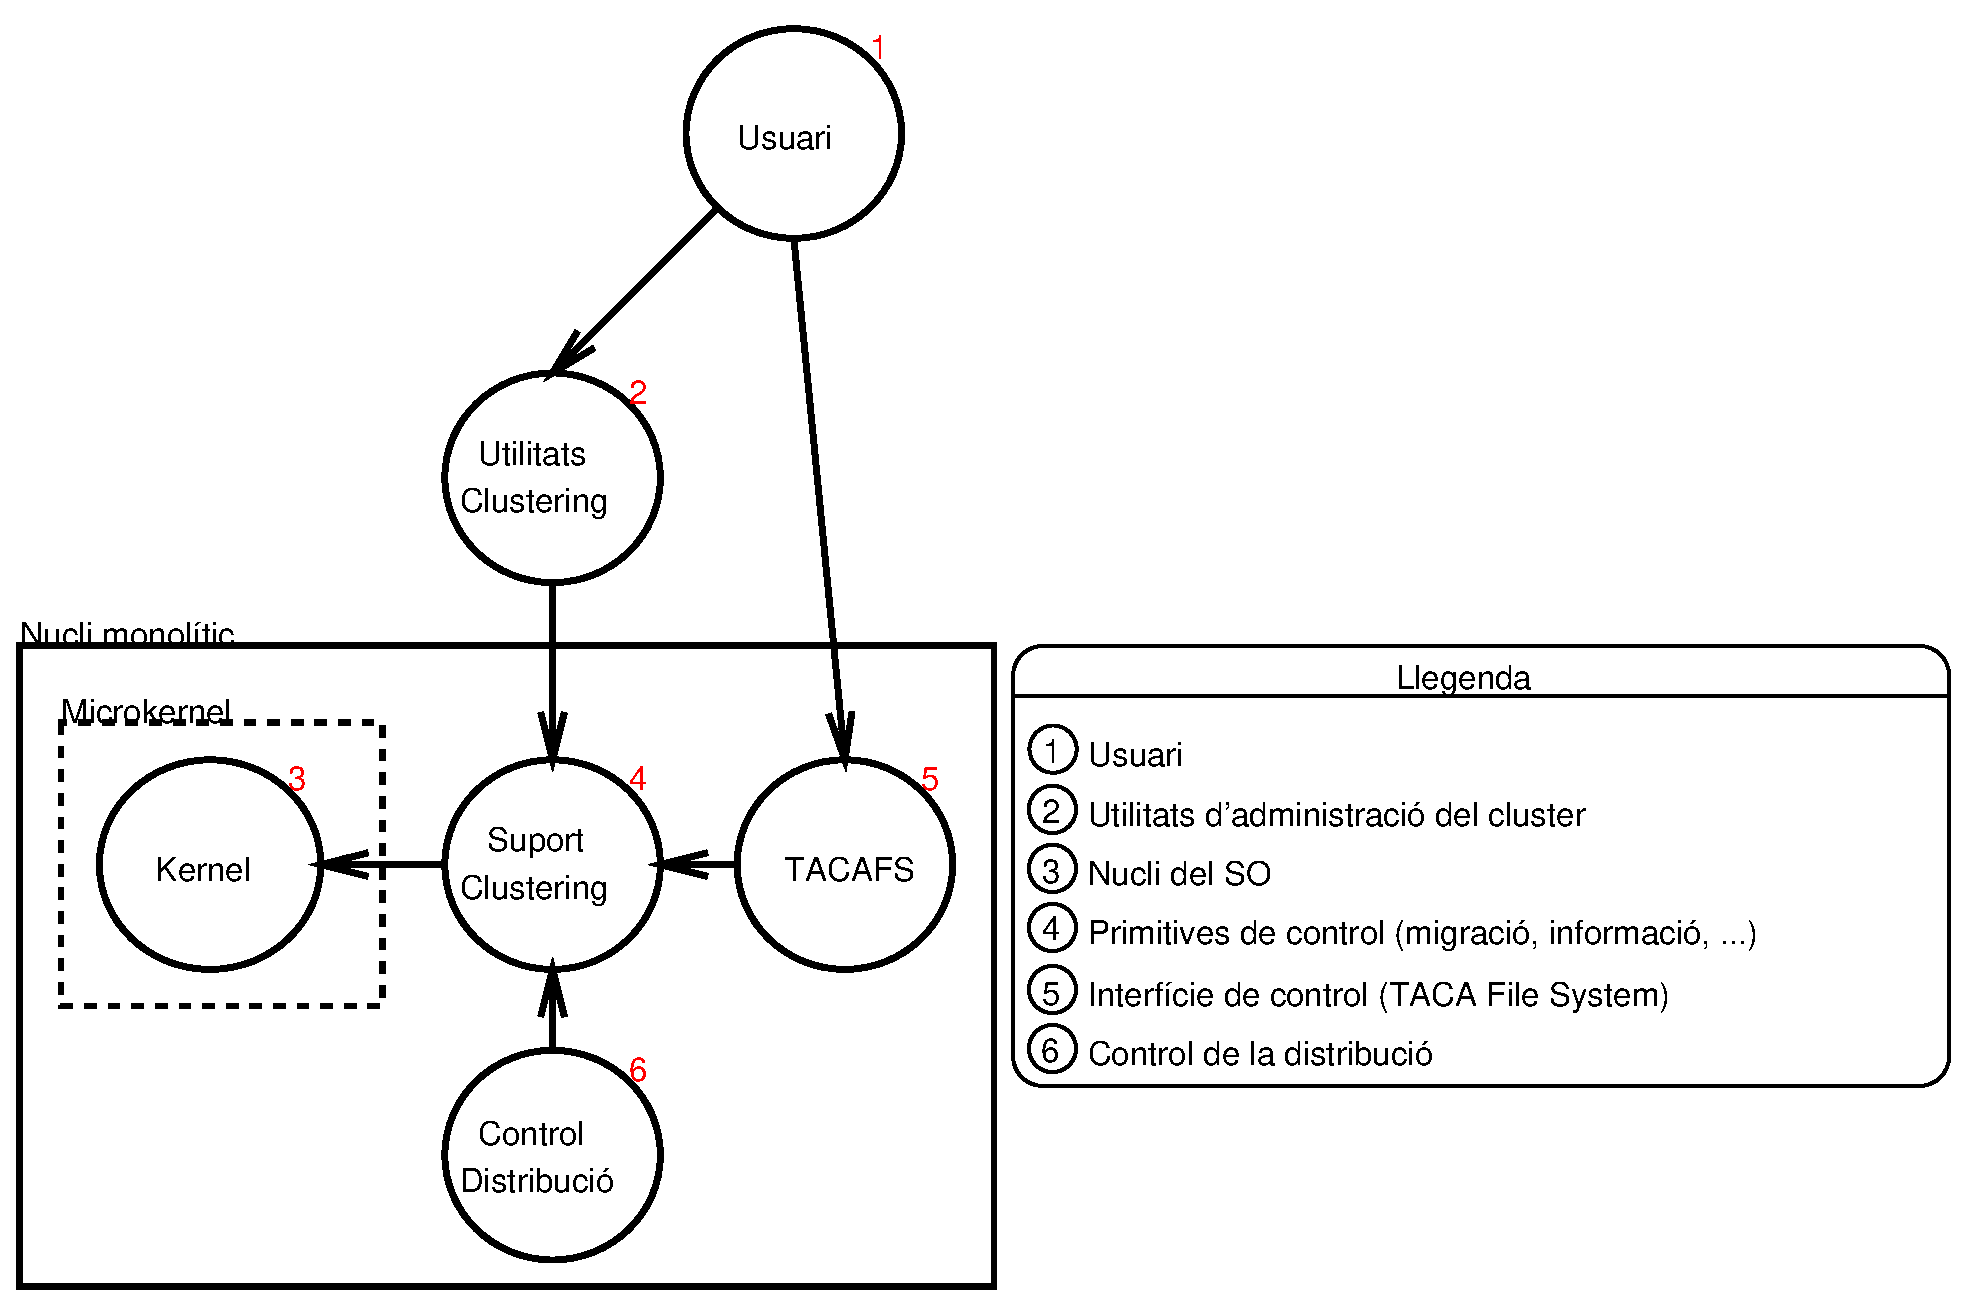
\includegraphics[scale=0.4]{esquema-supcl.eps}
   \caption{Esquema guay}
   \label{fig:esquema-supcl}
\end{figure}

\section{Soluci� super-guay}
En aquest disseny es tracta d'interectuar directament amb el nucli mitjan�ant
elsistema de fitxers virtual /proc.
Seguint amb l'exemple de migraci� de proc�s, en aquest cas es tractaria
d'escriure directament les dades necess�ries al fitxer corresponent del
directori /proc.En aquest cas escrivint el identificador de node al fitxer
"/proc/[PID]/goto" aconseguir�em migrar el proc�s de pid=PID al node desitjat. 

Aquest disseny, respecte l'anterior, aporta simplicitat i independ�ncia respecte
les utilitats que ofereix el cluster i les llibreries. Per� per contra s'hauria
de reescriure molt codi per exemple pel control d'errors, permisos, etc. que ja
estan implementats a les llibreries del software de clustering.

\section{...}


\nocite{lkAPI}

\chapter {Detalls d'implementaci�}

Per a fer la nostra implementaci�, hem escollit el \textit{disseny complex}.

Hem pres aquesta decisi� perqu� partint d'un escenari Linux-OpenMosix, no veiem
viables les altres opcions perqu� des de dins del propi kernel no es poden
executar aplicacions d'usuari com les OpenMosix Tools (\textit{disseny simple})
ni enlla�ar amb les llibreries corresponents (\textit{disseny intermig}), que
en el cas de OpenMosix, no s�n tals, sin� crides a sistema, que tampoc �s
possible utilitzar des de dins el kernel.

M�s tard, explicarem que les altres dues opcions realment si que s�n possibles.

A l'hora de crear la implementaci�, hem pensat en un objectiu molt concret per
tal de reduir el tamany de la implementaci� (doncs fer-la completa requereix
molt de temps i no �s l'objectiu d'aquesta pr�ctica).

Ens hem fixat com a objectiu la migraci� de processos entre nodes perqu� �s el
tret m�s significatiu del nostre programa.

Partint d'aquest objectiu hem estudiat quines s�n les m�nimes parts necess�ries
a implementar tant en el \textit{frontend} com en el \textit{backend}, pensant
que el projecte pugui ser ampliable a la resta del disseny que hem planificat.

Aix� doncs, el que hem implementat �s un \textbf{m�dul del kernel} que cont� les
seg�ents parts.


\section{Frontend: sistema de fitxers virtual}

\nocite{VFS-overview}
\nocite{VFS-kmp}
\nocite{VFS-lki}
\nocite{VFS-libfs}
\nocite{VFS-rkfs}
\nocite{VFS-lk}
\nocite{VFS-tlk}
Aquest sistema de fitxers est� basat en la interf�cie del VFS (\textit{Virtual
File System}) que proporciona Linux.

Al ser un sistema de fitxers virtual, tota la informaci� mostrada es genera de
forma din�mica amb les dades obtingudes del \textit{backend}.

B�sicament, en iniciar-se el m�dul, es registra el nostre sistema de fitxers:
\textit{tacafs}. I es desenregistra en descarregar el m�dul.

\begin{codi}
static int __init tacafs_init(void)
\{
   return register_filesystem(&tacafs_type);
\}

static void __exit tacafs_exit(void)
\{
   unregister_filesystem(&tacafs_type);
\}
\end{codi}

Seguidament a carregar el m�dul, ja es pot muntar el sistema de fitxers all� on
es vulgui, de forma que es crida a la operaci� que omple les dades del
\textit{super bloc}, que li associa l'inode que representa l'arrel del sistema
de fitxers.

Les funcions de m�s inter�s s�n les que van associades als fitxers i directoris.

Sobre els directoris, les funcions m�s destacables s�n:

\begin{description}
\item [file\_operations.readdir:]
Genera els continguts que es veuen en llegir els continguts d'un directori (per
exemple, els noms de fitxers, directoris i els seus permisos en fer un
\texttt{ls}).

En el seg�ent codi (\texttt{frontend/linux/*.c}) generem el contingut per al directori
arrel, que llista els clusters que hi ha al sistema. En la resta de directoris es
faria de forma an�loga per� canviant les crides al \textit{backend}.

\begin{codi}
int tacafs_f_readdir (struct file *file, void *dirent,
                      filldir_t filldir )
\{
   [...]
   if(filldir(dirent, ".", 1, file->f_pos++, de->d_inode->i_ino,
              DT_DIR)
      ||
      filldir(dirent, "..", 2, file->f_pos++,
              de->d_parent->d_inode->i_ino, DT_DIR))
      return 0;
   [...]
   num = num_clusters();      // CRIDA AL BACKEND
   [...]
   llistar_clusters(llista);  // CRIDA AL BACKEND
   while (llista != NULL) \{
      if(filldir(dirent, llista->nom, strlen(llista->nom),
                 file->f_pos++, DIR_INODE_NUMBER, DT_DIR))
         return 0;
      llista = llista->next;
   \}
   [...]
\}
\end{codi}

\item [inode\_operations.lookup:]
Donada una estructura dentry, que en el VFS de Linux �s l'encarregade de
representar la jerarquia de fitxers, i el inode pare al que pertany el dentry,
crea un inode, li associa les operacions corresponents, el mode i finalment
associa l'inode al dentry.

Aquesta funci� seria cridada en accedir al directori en q�esti�.

\begin{codi}
struct dentry *tacafs_i_lookup (struct inode *parent_inode,
                                struct dentry *dentry)
\{
   [...]
   if(!(file_inode = iget(parent_inode->i_sb, DIR_INODE_NUMBER)))
      return ERR_PTR(-ENOMEM);
   file_inode->i_mode = S_IFDIR|S_IRUSR|S_IWUSR|S_IRGRP|S_IROTH;
   // file_operations
   file_inode->i_fop = &tacafs_dir_fops;
   // inode_operations
   file_inode->i_op = &tacafs_iops;
   // afegir el inode al dentry
   d_add(dentry, file_inode);
\}
\end{codi}
\end{description}

En quant als fitxers, les operacions que duu associades s�n el \texttt{lookup},
que duu a terme la mateixa tasca que en el cas dels directoris, el \texttt{read}
i el \texttt{write} que s�n els encarregats de llegir i escriure els continguts
del fitxer i el \texttt{rename} que �s l'encarregat de tractar amb el moviment
de fitxers i directoris.

Les funcions \texttt{read} i \texttt{write} no ens ha calgut implementar-les per
l'objectiu que ens hem fixat.

La funci� clau per a la migraci� de processos �s \texttt{rename}, per� no la hem
pogut arribar a implementar degut a qu� ens hem trobat una s�rie de problemes
que ens han portat molt de temps per trobar-hi soluci� a l'hora d'implementar el
\textit{backend} d'OpenMosix que explicarem tot seguit.


\section{Backend: adaptaci� al sistema de clustering}

\subsection{Definici� de la interf�cie}

Partint dels objectius que ens hem fixat, hem definit una interf�cie gen�rica
(fitxer \linebreak \texttt{backend/backend.h}) per a tractar des del 
\textit{frontend} amb el \textit{backend}.

Aquesta interf�cie consta d'unes operacions necess�ries per a generar
l'estructura del sistema de fitxers:

\begin{codi}
int num_clusters();
int llistar_clusters (struct cluster_t *llista);
int num_nodes (struct cluster_t *cluster_id);
int llistar_nodes (struct cluster_t *cluster_id,
                   struct node_t *llista);
int num_procs (struct cluster_t *cluster_id, struct node_t *node_id);
int llistar_procs (struct cluster_t *cluster_id, struct node_t *node_id,
                   struct proces_t *lista);
\end{codi}

I una s�rie de funcions per a dur a terme les funcionalitats que hem definit:

\begin{codi}
int migrar (struct proces_t  *proces, struct node_t *node_desti);

/* El node pot rebre procs. nous ? */
int node_bloquejat_rebre (struct node_t *node);

/* El node pot enviar procs. nous ? */
int node_bloquejat_enviar (struct node_t *node);

/* El proces no es pot migrar */
int proces_bloquejat (struct proces_t *proc);
\end{codi}


\subsection{Implementacions de la interf�cie}

\subsubsection{Exemple \textit{dummy}}

Primerament hem implementat un petit \textit{backend} d'exemple que crea sempre
les mateixes dades per tal de comprovar que la part que hem implementat del
\textit{frontend} funciona correctament, �s a dir, tenim un sistema de fitxers
navegable.

Aquest exemple es troba a \texttt{backend/dummy/dummy.c}.


\subsubsection{El problema d'OpenMosix}

\nocite{OpenMosix-API}

El problema al que abans f�iem refer�ncia a l'apartat del \textit{frontend} �s
el que ens hem trobat a l'hora de fer una implementaci� per a OpenMosix.

B�sicament el problema �s que OpenMosix ha estat pensat per a ser accedit sola i
exclusivament a trav�s de la interf�cie que ofereix al directori
\texttt{/proc/hpc}, sense exportar cap s�mbol utilitzable des del propi nucli, de
forma que l'�nica manera d'accedir-hi �s a trav�s del VFS, el qual nom�s �s
accessible a trav�s de programes amb un context propi (com serien programes en
mode usuari o threads de kernel).

Aquest intent d'implementaci� es troba a \texttt{backend/openmosix/}.

Algunes possibles solucions que no hem pogut implementar per falta de temps
serien:

\begin{itemize}
\item
Una soluci� que hem trobat sense haver de modificar ni el kernel ni el codi
d'OpenMosix, �s, en tan bon punt s'activi el nostre sistema de fitxers, arrencar
un thread de kernel o programa en mode usuari (daemon) que esperi peticions
provinents del nostre \textit{backend}, moment en qu� aquest programa o thread
que duria a terme la petici� a trav�s de \texttt{/proc/hpc/} i retornaria el
resultat altra vegada al nostre \textit{backend} (veure la figura
\ref{fig:solucio-espai-usuari}).

\begin{figure}[hbtp]
   \centering
   \includegraphics[scale=0.3]{solucio-espai-usuari.eps}
   \caption{Esquema de la possible soluci�}
   \label{fig:solucio-espai-usuari}
\end{figure}

\item
Una altra soluci� molt menys elegant i m�s intrusiva seria exportar els s�mbols
de les funcions, dades i/o estructures que ens fessin falta del codi
d'OpenMosix, o b� afegir una part de codi propi que utilitzi el que hi ha a dins
d'OpenMosix i exportar aquestes funcions que ens proporcionarien just el que
volem, que seria com una extensi� del nostre \textit{backend} que entraria a
dins del codi del kernel.
\\
A m�s a m�s aquestes dues �ltimes solucions no s�n molt viables pel fet de qu� la
documentaci� d'OpenMosix tant externa com a dins del propi codi �s molt minsa.

\item
Una soluci� totalment circumstancial i depenent del binari seria la de con�ixer
un s�mbol exportat a partir del que, donat un offset fixe i conegut, es pugui
accedir a la zona que ens interessa.
\end{itemize}


\chapter{Possibles ampliacions al disseny}

\begin{description}
    \item \textbf{Utilitzaci� de diversos \textit{backend} alhora} \\
	Emulant el sistema que utilitza Linux per als diferents tipus de
	sistemes de fitxers, es podria incloure un sistema que
	permet�s registrar din�micament en forma de m�duls cadascun dels
	\textit{backend} sota demanda, de manera que en accedir a un cl�ster
	en el nostre arbre, se seleccionaria el \textit{backend} corresponent
	per a dur a terme la operaci� sol�licitada.

    \item \textbf{Recol�lecci� d'informaci� remota} \\
	Donades les limitacions d'\textit{OpenMosix} a l'hora d'accedir a la
	informaci� de nodes remots, es podrien implementar dos nous elements,
	un \textbf{recolector} d'informaci�, per a recollir la informaci� dels
	nodes remots, i un \textbf{informador}, que aniria a cadascun dels
	nodes remots als que volem poder accedir.

	Aix� doncs, la informaci� dels nodes remots seria la informaci� del
	node local d'all� on est� cadascun dels recolectors, salvant aix� el
	problema que ens oferia OpenMosix, i podent eliminar aleshores,
	tamb�, la limitaci� que nosaltres mateixos hem posat de crear
	processos des d'un sol node com a punt d'entrada.

    \item \textbf{Arquitectura transl�cida} \\
	A vegades es pot donar el cas de qu� un sistema de clustering concret
	proporcioni uns serveis molt espec�fics d'aquest, de forma que des del
	\textit{frontend} es podria oferir una interf�cie gen�rica que permet�s al
	\textit{backend} definir aquesta part m�s espec�fica de l'arbre de directoris.
	
	Aquesta soluci�, per�, requeriria que, en major o menor mesura, el mateix
	\textit{backend} proporcion�s les seves pr�pies funcions de generaci� de
	l'arbre espec�fic, proporcionant quelcom semblant a una versi� redu�da del
	\textit{frontend}.
	
	Duent-ho m�s enll�, per�, es podria arribar a crear una s�rie d'estructures i
	funcions gen�riques que evitessin aquesta feina a la capa d'abaix, tot i que
	un sistema de clustering sol anar molt lligat al sistema operatiu i, comparant
	les dues APIs de sistemes de fitxers que hem mirat (el VFS de Linux i el de
	GNU/Hurd), hem vist que, tret de petits detalls, les funcionalitats que
	ofereixen s�n les mateixes o molt similars, de manera que no seria molt
	dif�cil generalitzar-ne una interf�cie i amagar-ne els detalls en camps
	dedicats a la la informaci� espec�fica de cada sistema, tal com ja fa Linux,
	amb els sistemes de fitxers, que reserva un camp que �s un simple apuntador a
	dins dels inodes per a que cada sistema de fitxers hi posi la informaci� que
	consideri necess�ria.
\end{description}


\pagebreak 
\addcontentsline{toc}{chapter}{Bibliografia}
\bibliographystyle{plain} 
\bibliography{00-taca}

\end{document}          
